
%% BioMed_Central_Tex_Template_v1.06
%%                                      %
%  bmc_article.tex            ver: 1.06 %
%                                       %

%%IMPORTANT: do not delete the first line of this template
%%It must be present to enable the BMC Submission system to
%%recognise this template!!

%%%%%%%%%%%%%%%%%%%%%%%%%%%%%%%%%%%%%%%%%
%%                                     %%
%%  LaTeX template for BioMed Central  %%https://www.overleaf.com/project/5da486e90daa0200016ff561
%%     journal article submissions     %%
%%                                     %%
%%          <8 June 2012>              %%
%%                                     %%
%%                                     %%
%%%%%%%%%%%%%%%%%%%%%%%%%%%%%%%%%%%%%%%%%


%%%%%%%%%%%%%%%%%%%%%%%%%%%%%%%%%%%%%%%%%%%%%%%%%%%%%%%%%%%%%%%%%%%%%
%%                                                                 %%
%% For instructions on how to fill out this Tex template           %%
%% document please refer to Readme.html and the instructions for   %%
%% authors page on the biomed central website                      %%
%% http://www.biomedcentral.com/info/authors/                      %%
%%                                                                 %%
%% Please do not use \input{...} to include other tex files.       %%
%% Submit your LaTeX manuscript as one .tex document.              %%
%%                                                                 %%
%% All additional figures and files should be attached             %%
%% separately and not embedded in the \TeX\ document itself.       %%
%%                                                                 %%
%% BioMed Central currently use the MikTex distribution of         %%
%% TeX for Windows) of TeX and LaTeX.  This is available from      %%
%% http://www.miktex.org                                           %%
%%                                                                 %%
%%%%%%%%%%%%%%%%%%%%%%%%%%%%%%%%%%%%%%%%%%%%%%%%%%%%%%%%%%%%%%%%%%%%%

%%% additional documentclass options:
%  [doublespacing]
%  [linenumbers]   - put the line numbers on margins

%%% loading packages, author definitions

%\documentclass[twocolumn]{bmcart}% uncomment this for twocolumn layout and comment line below
\documentclass{bmcart}

%%% Load packages
%\usepackage{amsthm,amsmath}
%\RequirePackage{natbib}
%\RequirePackage[authoryear]{natbib}% uncomment this for author-year bibliography
%\RequirePackage{hyperref}
\usepackage[utf8]{inputenc} %unicode support
\usepackage{apacite}
\usepackage{appendix}
\usepackage{amsmath}
\usepackage{amsthm}
\usepackage{tikz}
\usetikzlibrary{arrows.meta}
\usetikzlibrary{shapes}
% for ASY interactive 3d figure
%\usepackage[inline]{asymptote}
\usepackage{amssymb} % for approx greater than
%\usepackage{caption}
\usepackage{placeins} % for \FloatBarrier
\usepackage{graphicx}
\usepackage{subcaption}
\usepackage{longtable}
\usepackage{setspace}
\usepackage{booktabs}
\usepackage{tabularx}
\usepackage{xcolor,colortbl}
\usepackage{chngpage}
\usepackage{natbib}
%\bibpunct{(}{)}{,}{a}{}{;} 
\usepackage{url}
\usepackage{nth}
\usepackage{authblk}
\usepackage[most]{tcolorbox}
\usepackage[normalem]{ulem}
\usepackage{amsfonts}
\usepackage{censor}
\usepackage{etoolbox}
\AtBeginEnvironment{quote}{\singlespace\small}
\AtEndEnvironment{quote}{\endsinglespace}
%\usepackage[applemac]{inputenc} %applemac support if unicode package fails
%\usepackage[latin1]{inputenc} %UNIX support if unicode package fails


%%%%%%%%%%%%%%%%%%%%%%%%%%%%%%%%%%%%%%%%%%%%%%%%%
%%                                             %%
%%  If you wish to display your graphics for   %%
%%  your own use using includegraphic or       %%
%%  includegraphics, then comment out the      %%
%%  following two lines of code.               %%
%%  NB: These line *must* be included when     %%
%%  submitting to BMC.                         %%
%%  All figure files must be submitted as      %%
%%  separate graphics through the BMC          %%
%%  submission process, not included in the    %%
%%  submitted article.                         %%
%%                                             %%
%%%%%%%%%%%%%%%%%%%%%%%%%%%%%%%%%%%%%%%%%%%%%%%%%


% Toggle show graphics
%\def\includegraphic{}
%\def\includegraphics{}



%%% Put your definitions there:
\startlocaldefs
\endlocaldefs


%%% Begin ...
\begin{document}

%%% Start of article front matter
\begin{frontmatter}

\begin{fmbox}
\dochead{Research}

%%%%%%%%%%%%%%%%%%%%%%%%%%%%%%%%%%%%%%%%%%%%%%
%%                                          %%
%% Enter the title of your article here     %%
%%                                          %%
%%%%%%%%%%%%%%%%%%%%%%%%%%%%%%%%%%%%%%%%%%%%%%

\title{Schemas of demographic time:\\ independent time measures can be informative}

%%%%%%%%%%%%%%%%%%%%%%%%%%%%%%%%%%%%%%%%%%%%%%
%%                                          %%
%% Enter the authors here                   %%
%%                                          %%
%% Specify information, if available,       %%
%% in the form:                             %%
%%   <key>={<id1>,<id2>}                    %%
%%   <key>=                                 %%
%% Comment or delete the keys which are     %%
%% not used. Repeat \author command as much %%
%% as required.                             %%
%%                                          %%
%%%%%%%%%%%%%%%%%%%%%%%%%%%%%%%%%%%%%%%%%%%%%%

\author[
   addressref={aff1, aff2},                   % id's of addresses, e.g. {aff1,aff2}
%   corref={aff1},                       % id of corresponding address, if any
%   noteref={n1},                        % id's of article notes, if any
   email={tim.riffe@gmail.com}   % email address
]{\inits{TR}\fnm{Tim} \snm{Riffe}}
\author[
   addressref={aff3, aff4},
   email={cohen@mail.rockefeller.edu}
]{\inits{JEC}\fnm{Joel E.} \snm{Cohen}}

%%%%%%%%%%%%%%%%%%%%%%%%%%%%%%%%%%%%%%%%%%%%%%
%%                                          %%
%% Enter the authors' addresses here        %%
%%                                          %%
%% Repeat \address commands as much as      %%
%% required.                                %%
%%                                          %%
%%%%%%%%%%%%%%%%%%%%%%%%%%%%%%%%%%%%%%%%%%%%%%

\address[id=aff1]{%                           % unique id
  \orgname{Ikerbasque: Basque Foundation for Science} % university, etc
 % \street{Plaza Euskadi 5},                     %
 % \postcode{48009}                                % post or zip code
 % \city{Bilbao},                              % city
 % \cny{ES}                                    % country
}
\address[id=aff2]{%                           % unique id
  \orgname{University of the Basque Country} % university, etc
 % \street{Barrio Sarriena, s/n},                     %
 % \postcode{48940}                                % post or zip code
 % \city{Leioa},                              % city
 % \cny{ES}                                    % country
}

\address[id=aff3]{%
  \orgname{The Rockefeller University}
 % \street{D\"{u}sternbrooker Weg 20},
 % \postcode{24105}
 % \city{Kiel},
 % \cny{Germany}
}
\address[id=aff4]{%
  \orgname{Columbia University}
  %\street{D\"{u}sternbrooker Weg 20},
  %\postcode{24105}
  %\city{Kiel},
  %\cny{Germany}
}

%%%%%%%%%%%%%%%%%%%%%%%%%%%%%%%%%%%%%%%%%%%%%%
%%                                          %%
%% Enter short notes here                   %%
%%                                          %%
%% Short notes will be after addresses      %%
%% on first page.                           %%
%%                                          %%
%%%%%%%%%%%%%%%%%%%%%%%%%%%%%%%%%%%%%%%%%%%%%%

\begin{artnotes}
%\note{Sample of title note}     % note to the article
%\note[id=n1]{Equal contributor} % note, connected to author
\end{artnotes}

\end{fmbox}% comment this for two column layout

%%%%%%%%%%%%%%%%%%%%%%%%%%%%%%%%%%%%%%%%%%%%%%
%%                                          %%
%% The Abstract begins here                 %%
%%                                          %%
%% Please refer to the Instructions for     %%
%% authors on http://www.biomedcentral.com  %%
%% and include the section headings         %%
%% accordingly for your article type.       %%
%%                                          %%
%%%%%%%%%%%%%%%%%%%%%%%%%%%%%%%%%%%%%%%%%%%%%%

\begin{abstractbox}

\begin{abstract} % abstract
\parttitle{Background} 
[JOEL OFFERS TO REWRITE THIS ABSTRACT AFTER THE MAIN TEXT MATURES, BUT WOULD ALSO 
WELCOME A DRAFT BY TIM IF TIM WISHES TO DRAFT A REVISED ABSTRACT.]
%The demographic time identity consists in a linear relationship between all pairs of six fundamental time measures: age, period, cohort, time to death, length of life, and time of death. Certain subsets of time measures in this and other higher order identities consist in time measures that are independent of one another.
\parttitle{Objective} 
%We aim to clarify the relationship between independent time measures and the identities within which they are nested, with special attention to the demographic time identity and its three independent time dyads. We also aim to determine whether data structured on such time dyads might be useful in demographic research.
\parttitle{Data and Methods} 
We illustrate concepts visually based on disability prevalence data estimated from the US Health and Retirement study. 
%We display and evaluate several varieties of prevalence surfaces.
\parttitle{Results} 
%We show that a Cartesian mapping of independent time dyads forms a redundant mapping of the demographic timespace. These add three novel demographic perspectives to four previously described Lexis-like perspectives, for a total of seven proposed standard perspectives. 
\parttitle{Conclusions} 
%We show independent sets of time measures to be consistent with the temporal identities within which they are nested. We demonstrate that these perspectives can be useful for pattern detection and characterization in demographic research.
\end{abstract}

%%%%%%%%%%%%%%%%%%%%%%%%%%%%%%%%%%%%%%%%%%%%%%
%%                                          %%
%% The keywords begin here                  %%
%%                                          %%
%% Put each keyword in separate \kwd{}.     %%
%%                                          %%
%%%%%%%%%%%%%%%%%%%%%%%%%%%%%%%%%%%%%%%%%%%%%%


\begin{keyword}
\kwd{age structure}
\kwd{data visualization}
\kwd{age-period-cohort}
\kwd{disability prevalence}
\end{keyword}

% MSC classifications codes, if any
%\begin{keyword}[class=AMS]
%\kwd[Primary ]{}
%\kwd{}
%\kwd[; secondary ]{}
%\end{keyword}

\end{abstractbox}
%
%\end{fmbox}% uncomment this for twcolumn layout

\end{frontmatter}

%%%%%%%%%%%%%%%%%%%%%%%%%%%%%%%%%%%%%%%%%%%%%%
%%                                          %%
%% The Main Body begins here                %%
%%                                          %%
%% Please refer to the instructions for     %%
%% authors on:                              %%
%% http://www.biomedcentral.com/info/authors%%
%% and include the section headings         %%
%% accordingly for your article type.       %%
%%                                          %%
%% See the Results and Discussion section   %%
%% for details on how to create sub-sections%%
%%                                          %%
%% use \cite{...} to cite references        %%
%%  \cite{koon} and                         %%
%%  \cite{oreg,khar,zvai,xjon,schn,pond}    %%
%%  \nocite{smith,marg,hunn,advi,koha,mouse}%%
%%                                          %%
%%%%%%%%%%%%%%%%%%%%%%%%%%%%%%%%%%%%%%%%%%%%%%

%%%%%%%%%%%%%%%%%%%%%%%%% start of article main body
% <put your article body there>

\section*{Background}
Demography is concerned with populations of lives in time. 
The purpose of this article is to revise, simplify, and extend
an approach to measures of demographic time developed by \citet{riffe2017demographictime},
and to illustrate this revised approach by an empirical 
example (the United States Health and Retirement Survey).


Demography generally characterizes
demographic time on an infinite real line with no absolute origin.
In the language of measurement theory, the demographic time line is an interval scale,
not a ratio scale.
For example, 
the calendar year 2000 is not twice as big as the calendar year 1000, it is simply a thousand years later.
The year 1900 is as different from 1800 as the year 2000 is from 1900, 
though the ratios of these two pairs of times differ.
Creationists notwithstanding, there is no natural point of origin for demographic time.
By contrast, on the scale of absolute temperature or thermal energy,
2000 kelvin is twice 1000 kelvin, 
and 1000 kelvin is twice 500 kelvin, 
because both are measured on a ratio scale from absolute zero.

Demography distinguishes points from intervals. 
Points are exemplified by a time of birth, the present, or a time of death.
An interval is the distance between two distinct points. 
For example, the interval from time of birth to time of death is length of life. 

In practice,
the distinction between points and intervals is less clear than the words suggest, and 
depends on the time-scale of interest.
For example, in one context a calendar year may be treated as a point in time (for the year of birth of a birth cohort) 
while in another context a calendar year may be treated as an interval (for a crude birth rate, the number of births per year).
The applied context usually makes clear the distinction between points and intervals.

\section*{Representations of demographic time by directed graphs and linear algebra}

Points of demographic interest in each life include its time of birth 
(denoted $C$ for ``cohort''), its time of death (denoted $D$), and the period (denoted $P$).
These points are the focus of this section.
Other points are discussed in the following section.
By abuse of notation, we shall use the same letter to refer to the \emph{name}
of a point in time and to the numerical \emph{value} of that point on the time line.
With this convention,
it makes sense to compare the numerical value of two named points. 
For example, to qualify as a life in demography, points $C$ and $D$ must satisfy $C < D$.
In this section we assume that $C<P<D$.
We suggest other possible relations of $P$ to $C$ and $D$ in the following section.




Every interval $\Delta$ is defined by a pair of points: $\Delta =$ (starting point $\Delta_1$, ending point $\Delta_2$). 
The length of an interval is the time value of the 
ending point minus the time value of the starting point: $|\Delta| =\Delta_2 - \Delta_1$ .
For example, exactly three intervals (no more, no fewer) of positive length are implied by the three points $C, P, D$ under the assumption that $C<P<D$. 
These intervals are age $A=(C,P)$ with length $|A|=P-C$ at period $P$; 
remaining time to death $T=(P,D)$ with length $|T|=D-P$ at period $P$; 
and length of life $L=(C,D)$ with length $|L|=D-C$ (regardless of the period $P$).
Because we assume $C<P<D$, these three intervals all have positive length.
The intervals $A,T,L$ are not independent because they are constrained by the same set of three points,
as \citet{riffe2017demographictime} noted.
They must obey $|A|+|T|=|L|$
because $|A|+|T|=(P-C)+(D-P)=D-C=|L|$.


This structure of a finite set of points on a line and intervals between pairs of those points
is described by two areas of mathematics, weighted directed graphs and linear algebra. 
These two descriptions are intimately related, not surprisingly, because they describe the same subject.
We now present weighted directed graphs and the corresponding linear algebra using the example of the
set of points $\{C,P,D\}$ and intervals $\{A,T,L\}$ assuming $C<P<D$.

A weighted directed graph (Fig. \ref{fig:digraph}) consists of a set of vertices (here $\{C,P,D\}$), 
a set of directed edges or arrows (here $\{A,T,L\}$), 
and a set of weights, one for each arrow (here $\{|A|,|T|,|L|\}$).


\begin{figure}[h!]
 \captionsetup{width=.8\linewidth}
\centering
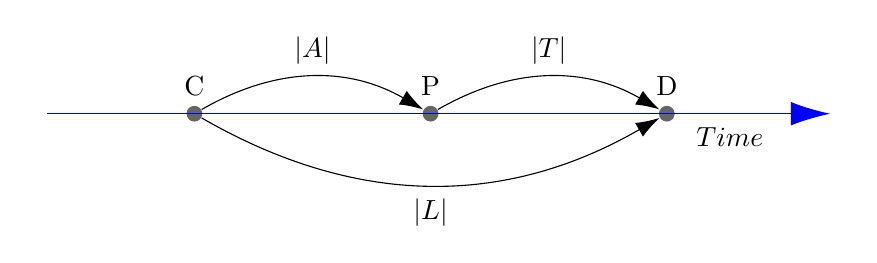
\begin{tikzpicture}[roundnode/.style={circle, fill=black!60, inner sep=0pt, minimum size=2mm}]
\tikzset{edge/.style = {->}}
\node[roundnode, label = C] (C) at  (0,0) {};
\node[roundnode,label = P] (P) at  (3,0) {};
\node[roundnode,label = D] (D) at  (6,0) {};
\node[] (X) at (-2,0) {};
\node[] (Z) at (8.2,0) {};
\node[] (a) at (1.5,.8) {$|A|$};
\node[] (t) at (4.5,.8) {$|T|$};
\node[] (l) at (3,-1.25) {$|L|$};
\node[] (c) at (6.8,-.3) {$Time$};
\draw[-{Latex[width=2mm, length = 3mm]}] (C) to[bend left](P);
\draw[-{Latex[width=2mm, length = 3mm]}] (P) to[bend left] (D);
\draw[-{Latex[width=2mm, length = 3mm]}] (C) to[bend right] (D);
\draw[-{Latex[width=3mm, length = 5mm]},blue] (X) to (Z);
%\draw[edge] (c) to (d);
\end{tikzpicture}
%\includegraphics[width=4.5in]{Figures/Fig1DirectedGraph20210530.pdf}
\caption{Directed graph of three time points $\{C,P,D\}$
and three time intervals $\{A,T,L\}$, with arrows
weighted by interval length, assuming that $C<P<D$.}
\label{fig:digraph}
\end{figure}

An algebraic equivalent of a directed graph is an incidence matrix
(exemplified by $M$ below).
The incidence matrix of a directed graph has one row for each arrow (or interval)
and one column for each vertex (or point).
In the row corresponding to an interval $\Delta =$ (starting point, ending point),
the element in the column corresponding to the starting point is $-1$ and
the element in the column corresponding to the ending point is $1$.
All other elements in the row corresponding to interval $\Delta$ are $0$.

For example, the incidence matrix of the weighted directed graph
with vertices $\{C,P,D\}$, 
arrows $\{A,T,L\}$, 
and corresponding weights $\{|A|,|T|,|L|\}$ is
\[
M = \bordermatrix{~ & C & P & D \cr
A & -1 & 1 & 0 \cr
T & 0 & -1 & 1 \cr
L & -1 & 0 & 1 \cr}
.\]

If we arrange the points $\{C,P,D\}$ in a vector $V$ in the same order that we used to order the columns of $M$,
\[
V =
\begin{pmatrix}
C \\
P \\
D \\
\end{pmatrix}
,\]
%\[
%V = \bordermatrix{~  \cr
%~ & C \cr
%~ & P \cr
%~ & D \cr}
%,\]
then the vector $W$ of weights (i.e., interval lengths) equals the matrix $\times$ vector product $W=M\cdot V$:
\begin{align}%\label{eq:WequalsMV}
%\[
W =
\begin{pmatrix}
|A| \\
|T| \\
|L| \\
\end{pmatrix}
=
\begin{pmatrix}
P-C \\
D-P \\
D-C \\
\end{pmatrix}
=&
\begin{pmatrix}
 -C & +P & +0\cdot D \\
 0\cdot C & -P & +D \\
-C & +0\cdot P & +D \\
\end{pmatrix} \notag \\ 
 =&
\begin{pmatrix}
 -1 & +1 & 0 \\
 0 & -1 & +1 \\
 -1 & 0 & +1 \\
\end{pmatrix}
\cdot
\begin{pmatrix}
C \\
P \\
D \\
\end{pmatrix}
= M\cdot V.\label{eq:WequalsMV}%\]
\end{align}
The equation $W=M\cdot V$ succinctly combines the three linear equations for $|A|,|T|,|L|$ stated 
in \eqref{eq:WequalsMV}.
Given any two elements of any one of these three equations, the third element of that equation is specified. 
For example, age $|A|$ and period $P$ determine cohort $C$;
$|A|$ and $C$ determine $P$; and $P$ and $C$ determine $|A|$.

Equation \eqref{eq:WequalsMV} gives all the information required to construct the 
weighted directed graph (Fig. \ref{fig:digraph}) and vice versa: 
the two descriptions are mathematically equivalent.

Every row of $M$ is some linear combination of the remaining two rows of $M$.
Specifically, the first row is the third minus the second;
the second row is the third row minus the first;
and the third row is the first row plus the second.
Thus the three linear equations contained in $W=M\cdot V$
are said to be linearly dependent.
%JOEL HERE Give the directed graph, , the incidence matrix, the linear algebra. Then go to Riffe et al. 2017
%\[
%\begin{matrix}
%-1 & 3 \\
%2 & -4
%\end{matrix}
%=
%\begin{pmatrix}
%-1 & 3 \\
%2 & -4
%\end{pmatrix}
%\]

%Dated events on a timeline form the foundation of numerous empirical approaches to detect, estimate, and describe patterns in processes and outcomes in the social sciences. Processes may be continuous/discrete, conditional/unconditional, forward/backward \citep{brouard2019backward}, or others. Outcomes may be prevalence, expectancies and variances, sequences, episode statistics, and others. Outcomes can be calculated from a process model or directly from data. Examples of process patterns include age-structured rates of fertility, mortality, and migration. Examples of outcome patterns include trends in length of life, healthy life expectancy, counts of births structured in some way, or employment trajectories. 
%
%This paper deals with the calendar relationships that underpin all such knowledge of the world. Most empirical work that describes processes and outcomes makes use of a limited subset of the temporal structure that is available, and often the implications of relationships between time measures are unrecognized. 

%Previous work \citep{riffe2017demographictime} formalizes the relationship between events in time, and the durations between events. A set of events determines a further set of durations. A set of events and their implied durations comprise a relationship that we call a temporal \emph{identity}. The most common of these in empirical demographic research is the \emph{Lexis} identity between period (date), birth cohort (date), and age (duration): $C + A = P$. Many other Lexis-like relationships between linearly dependent time measures can be combined into higher-order Lexis identities. 
%
%A primary example of a higher-order Lexis identity is the so-called \emph{demographic time identity}, which defines relationships among age (A), period (P), cohort (C), time until death (T), time of death (D), and length of life (L). 

In describing the relationships among the points 
$\{C,P,D\}$ and the intervals $\{A,T,L\}$, 
\citet{riffe2017demographictime} distinguish what they call \emph{informative} dyads from what they call \emph{uninformative} dyads. 
They define an informative dyad as any pair of two points, two intervals, or one point and one interval from the set $\{C,P,D,A,T,L\}$
that determines some third member of this set.
For example, $A$ and $L$ determine $T$.
\citet{riffe2017demographictime} define an uninformative dyad as any pair of two points, two intervals, or one point and one interval 
from the set $\{C,P,D,A,T,L\}$ that
does \emph{not} determine any third member of this set. 
They give three examples: $\{P,L\},\{D,A\}$, and $\{C,T\}$.
\citet{riffe2017demographictime} observe that there are no other such so-called 
``uninformative'' dyads from the set $\{C,P,D,A,T,L\}$
and that each such dyad contains one point and one interval from the set $\{C,P,D,A,T,L\}$.
In each case, the point is not part of the definition of the interval: 
for example, $P$ is not part of the definition of $L=(C,D)$.


%, which are depicted in the authors' Tab.~(2) and discussed in the text as follows:
%\begin{quote}
%Triad identities are more meaningful than uninformative dyads. This is so even in the absence of data, due to the underlying relationship between measures. Each of the triad identities can accommodate some version of a lifeline, for instance \citep[p5][]{riffe2017demographictime}. 
%\end{quote}

Here we propose that what \citet{riffe2017demographictime} call an uninformative dyad might better be called
an \emph{independent} dyad.
We now give three hypothetical examples to show how
such a pair can reveal meaningful relationships in data. 
In these examples, we assume we are given a population of people
for each of whom we know the date $C$ of birth and the date $D$ of death.
In a later section,
we give an illustrative empirical example using 
disability prevalence patterns estimated from the US Health and Retirement Study. 


The first example considers the independent dyad consisting of the point $P$ (period)
and the interval $L$ (life length).
We pick a sequence of values of the period $P$ 
(e.g., the individual years in the nineteenth century, from $P_1=1801$ to $P_2=1900$)
and for each $P$ in the interval $[P_1, P_2]$
we select all those lives who were born before the selected $P$ and who died after $P$, 
so that $C<P<D$.
We also pick a sequence of values of life length $L$
(e.g., completed years of life from $L_1=0$ to $L_2=125$).
Over the rectangle $[P_1, P_2] \times [L_1, L_2]$ in the $(P,L)$-plane,
that is, the plane with abscissa ($x$-axis) $P$ and ordinate ($y$-axis) $L$,
we tabulate a histogram (frequency distribution) of lives.
Specifically, on the third dimension ($z$-axis) over the year $\times$ year box at each $(P,L)$,
we mark the number $N(P,L)$ of lives alive at $P$ whose life length at their death is $L$.

For each period $P$ (each calendar year in the nineteenth century, for example),
the sum $N(P,+)$ of the counts over all life lengths $L$ 
(from 0 to 125, for example) is the population size alive at year $P$.
Also, for each life length $L$,
the sum $N(+,L)$ of the counts over all periods $P$ (from $P_1=1801$ to $P_2=1900$, for example)
is the number of years of life lived during the interval $[P_1, P_2]$ by people who died at age $L$.
For each $P$, the ratios $N(P,L)/N(P,+), L=L_1, L_1+1, \ldots, L_2$ are 
the probability distribution of length of life at period $P$.
Improving mortality would be signaled by a shift in the probability mass toward longer life lengths $L$
with increasing period $P$.
Similarly, for each $L$, the ratios $N(P,L)/N(+,L), P=P_1, P_1+1, \ldots, P_2$ are the probability distribution of 
years of life lived during the interval $[P_1, P_2]$ by people who die at age $L$.
For a given $L$, an increasing trend in the ratios $N(P,L)/N(+,L)$ with increasing $P$ could
signal population growth, changing age structure, and/or improving survival.
However, if the ratios $N(P,L^+)/N(+,L^+)$ 
increase for longer lives $L^+$ 
while the ratios $N(P,L^-)/N(+,L^-)$ decrease for shorter lives $L^-<<L^+$,
the trends 
signal improving survival at older ages combined with an older age structure.
(We do not dwell on a third, obvious normalization. 
The probability distribution $N(P,L)/N(+,+), P=P_1, P_1+1, \ldots, P_2; L=L_1, L_1+1, \ldots, L_2$,
where $N(+,+)$ is the sum of the frequency counts over all periods $P$ and all life lengths $L$, 
has the same shape as the histogram of counts $N(P,L)$.)

[TIM, PLEASE CHECK THIS PARAGRAPH ESPECIALLY CAREFULLY TO MAKE SURE THAT IT MAKES SENSE.]
The second example considers the independent dyad consisting of the point $D$ (time of death)
and the interval $A$ (age).
Following the method of the first example, over the $(x,y)$-plane $(D,A)$, we construct the frequency distribution in which
$N(D,A)$ is the number of individuals who die in year $D$ and who are of age $A$
at the (unstated) period $P$.
Then the sum $N(D,+)$ of $N(D,A)$ over all ages $A$ is the total number of individuals of any age
who die in year $D$.
For each $D$, the set of ratios $N(D,A)/N(D,+)$ gives,
at the (unstated) period $P$,
the probability distribution of the population by age, or the age structure,
of the people who die in year $D$.
Also, $N(+,A)$ is the total of number of people at age $A$ at the (unstated) period $P$ summed over all years of death $D$.
Since each person has a unique year of death, no one is counted twice. 
For each $A$, the set of ratios $N(D,A)/N(+,A)$ shows the distribution over years of death $D$ of individuals aged $A$ at the (unstated) period $P$.


The third example considers the independent dyad consisting of the point $C$ (time of birth)
and the interval $T$ (time to death).
As before, over the $(x,y)$-plane $(C,T)$, we construct the frequency distribution in which
$N(C,T)$ is the number of individuals born in year $C$ who have $T$ 
years of remaining life at the (unstated) period $P$.
Such individuals may have differing ages and life lengths.
Then the sum $N(C,+)$ of $N(C,T)$ over all $T$ is the number of individuals born in year $C$
and alive at the (unstated) period $P$.
The probability distribution given by $N(C,T)/N(C,+), T=0, 1, \ldots$
shows the distribution of remaining life length among people born in year $C$
and alive at the (unstated) period $P$.
If, as $C$ increases, the probability distribution given by $N(C,T)/N(C,+)$ has increasing probability mass
at higher remaining lifetimes $T$, then survival of the elderly is improving.


%CT plane
%The thanatological age distribution of a birth cohort specifies that birth cohort's life table (distribution of T given C).
%Conversely, the distribution of birth cohorts of people of a given thanatological age reveals mortality history and inequalities in survival. If more of the people who will die in 5 years are from recent cohorts than from cohorts long ago, this population has high childhood mortality and low survival to old ages.
%
%AD plane
%For a given age A, the distribution of the death cohort D of individuals gives the conditional life table, conditional on reaching the given age A, and hence gives, for example, the remaining life expectancy and the variability of remaining life, among other summaries of the conditional life table.
%Conversely, for a given death cohort D, the distribution of age A of individuals specifies the distribution of their birth cohorts and life lengths.


%For better semantics and precision, we suggest calling these \emph{independent} dyads rather than uninformative dyads. We relate independent dyad diagrams to lifelines in two dimensions (2d). We relate 2d independent planes to the three-dimensional (3d) demographic time identity, showing how these are also cross-sections of the same 3d volume, but which follow a cubic rather than a tetrahedral structure. We show how data structured on independent time measures may still reveal meaningful patterns using 
%We speculate on how data structured by independent time measures may be meaningful in general.

%\section*{Geometric relationships}
%
%The demographic time identity can be represented as a tetrahedral graph, with time measures mapped to the six edges of a tetrahedron. The four Lexis-like identities are found on the faces of the tetrahedron. The identity fills a 3d space because tetrahedra tessellate with octahedra in a 2:1 ratio. \citet{riffe2017demographictime} considered neither independent pairs of time measures nor the significance of octahedra in this geometric construct. Figure~\ref{fig:tet} shows the tetrahedral graph of the demographic time identity among age (A), period (P), cohort (C), time to death (T), death cohort (D), and length of life (L). Independent dyads are those that do not share any vertex in the graph, and these appear as disjoint and perpendicular in the present 2d graph representation, though they are not perpendicular in 3d space: CT, LP, and AD.
%
%\begin{figure}[h!]
%\centering
%\includegraphics[width=4in]{Figures/TetraHedronEdgesOnly.pdf}
%\caption{Tetrahedral graph of demographic time hexad identity, with edges
%labelled by the six time indices. Reproduced from 
%\citet{riffe2017demographictime}.}
%\label{fig:tet}
%\end{figure}
%
%In a triad identity there are no independent dyads, but in the demographic time identity there are three independent dyads, each consisting in an event paired with a duration defined as the interval between the other two dated events. In general, a time identity defined on the basis of $n$ events implies a graph with $n+1$ vertices, implying a total of $\binom{n+1}{2}$ graph edges; see \citet{riffe2017demographictime} for multiple examples, though not formal proof. Each edge in the graph represents a time measure. Since $n$ of the edges are calendar-event measures, $\binom{n+1}{2} - n$ are duration measures. The $n$ calendar-dated measures are represented as graph edges sharing a single vertex. Triad identities are found wherever two edges share a vertex, for a total of three vertices, which means there must be $\binom{n+1}{3}$ of them within an identity. Independent dyads are pairs of edges that do not share a vertex, meaning that they use four vertices. Since there are $\binom{n+1}{2}$ ways to select one edge, there are $\binom{n-1}{2}$ ways to do so after having removed the two vertices of the first edge, or $\frac{1}{2}\binom{n+1}{2}\binom{n-1}{2}$ unique ways to select two unconnected edges, which simplifies to $3\binom{n+1}{4}$ independent dyads. For a more complicated example, a multistate model of period, birth, marriage, divorce, and death ($n=5$) would therefore imply 45 independent dyads, and a total of 20 triad identities. As $n$ increases, the fraction of possible temporal dyads that are independent approaches 1. To illustrate this point think of the universe of all dates and the potential durations between them: Pick two out of this massive urn and they will almost certainly be independent in this sense.
%
%Any pair of quantitative variables can define the axes of a standard Cartesian plane. When Cartesian axes are defined by two independent time measures and in equal time units, the resultant plane is an isometric projection. Let's call this an independent plane for short. There are two ways that an independent plane may be treated: either (i) accounting for a larger temporal identity or (ii) not. For the first kind (i) planes are cross-sections of the same 3d demographic timespace previously defined in Fig.~\ref{fig:tet}, and the independent dyads can also be conceived of as \emph{axes of view} on the demographic timespace. This idea is described further in Sec.~\ref{sec:viewaxes}. For the second kind (ii), independent planes are the same as any standard Cartesian plane used in data analyses: patterns revealed in data could be due to real structure or due to sample heterogeneity in other time measures. That is, the larger temporal identity within which these independent measures are nested is \emph{flattened}. Here we limit comments to the 3d case of the demographic time identity.
%
%\subsection*{View axes}
%\label{sec:viewaxes}
tikz%
%\begin{figure}
%\begin{subfigure}[t]{0.45\linewidth}
%    \centering
%    %\input{ASY/DepViewAxes.tex}
%    \resizebox{\linewidth}{\linewidth}{
%    

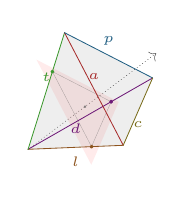
\begin{tikzpicture}[line join = round, line cap = round]

\coordinate (A) at (0.8737734,0.4020789,0.2735919); % incident to DPC (event node)
\coordinate (B) at (-0.5404401,0.6813372,-0.493664); % incident to TPA (step clocks!)
\coordinate (C) at (0.1666667,-0.787218,-0.5937256); % incident to LAC (origin anchor)
\coordinate (D) at (-0.5,-0.2961981,0.8137977); % incident to TLD (destination anchor)


% median lines: pick one
% \draw[->,color={rgb:red,1;green,1;blue,1}, densely dotted, line width = {0.2pt}] (A) -- (3*-0.2912578, 3*-0.1340263, 3*-0.0911973); % $TAL$ median
% \draw[->,color={rgb:red,1;green,1;blue,1}, densely dotted, line width = {0.2pt}] (B) -- (3*0.1801467, 3*-0.2271124, 3*0.1645547); % CDL median
% \draw[->,color={rgb:red,1;green,1;blue,1}, densely dotted, line width = {0.2pt}] (C) -- (3*-0.0555556, 3*0.262406, 3*0.1979085); % TPD median;
\draw[->,color={rgb:red,1;green,1;blue,1}, densely dotted, line width = {0.2pt}] (D) -- (3*0.1666667, 3*0.0987327, 3*-0.2712659); % APC median;

% bimedian lines: pick one
% \draw[->,color={rgb:red,1;green,1;blue,1}, densely dotted, line width = {0.2pt}] (1.3*-0.16666665,1.3*-0.54170805,1.3*0.11003605) -- (1.3*0.16666665,1.3*0.54170805,1.3*-0.11003605); % $LP$ bimedian
% \draw[->,color={rgb:red,1;green,1;blue,1}, densely dotted, line width = {0.2pt}] (1.3*-0.1868867,1.3*-0.0529404,1.3*-0.5436948) -- (1.1*0.1868867,1.3*0.0529404,1.3*0.5436948); % $AD$ bimedian
% \draw[->,color={rgb:red,1;green,1;blue,1}, densely dotted, line width = {0.2pt}] (1.3*-0.52022005,1.3*0.19256955,1.3*0.16006685) -- (1.3*0.52022005,1.3*-0.19256955,1.3*-0.16006685); % $TC$ bimedian

% redish transparent independent plane passing through midpoint 
% (match to bimedian line)
% bimed plane
%\fill[-, fill={rgb:red,1;green,0;blue,0}, opacity=.08] (0.7283081,-0.2695973,-0.2240936)--(0.2616414,0.0741166,0.7611727)--(-0.7283081,0.2695973,0.2240936)--(-0.2616414,-0.0741166,-0.7611727)--cycle; 

 % bimed intersection plane
%\draw[-, color={rgb:red,1;green,1;blue,1}, opacity=.5, line width = {0.1pt}] (0.5202201,-0.1925695,-0.1600669)--(0.1868867,0.0529404,0.5436948)--(-0.5202201,0.1925695,0.1600669)--(-0.1868867,-0.0529404,-0.5436948)--cycle;
% 0,0,0
%\node[mark size=.3pt,color={rgb:red,1;green,1;blue,1}, opacity=.5] at (0,0,0) {\pgfuseplotmark{*}}; 


% redish transparent triad plane passing through midpoint 
% (match to median line)
% med plane
\fill[-, fill={rgb:red,1;green,0;blue,0}, opacity=.08] (0.5821886,0.2370479,0.6351246)--(-0.7377441,0.4976889,-0.0809808)--(-0.0777778,-0.8729626,-0.1743716)--cycle; 

 % med intersection plane
\draw[-, color={rgb:red,1;green,1;blue,1}, opacity=.5, line width = {0.1pt}] (0.415849,0.1693199,0.4536605)--(-0.5269601,0.3554921,-0.0578434)--(-0.0555556,-0.6235447,-0.1245512)--cycle;
% tri centroid:
\node[mark size=.3pt,color={rgb:red,1;green,1;blue,1}, opacity=.5] at (-0.05555556,-0.0329109,0.09042196) {\pgfuseplotmark{*}}; 





% light shaded faces
\fill[-, fill={rgb:red,1;green,1;blue,1}, opacity=.05] (A)--(D)--(B)--cycle;       % TDP
\fill[-, fill={rgb:red,1;green,1;blue,1}, opacity=.05] (A)--(D)--(C)--cycle;       % CDL
\fill[-, fill={rgb:red,1;green,1;blue,1}, opacity=.05] (B)--(D)--(C)--cycle;       % TAL
\fill[-, fill={rgb:red,1;green,1;blue,1}, opacity=.05] (A)--(B)--(C)--cycle;       % APC

% color edges
\draw[-, color ={rgb:red,136;green,31;blue,147}, line width = {0.3pt}] (A)--(D);   % D
\draw[-, color ={rgb:red,197;green,117;blue,43}, line width = {0.3pt}] (D)--(C);   % L
\draw[-, color ={rgb:red,78;green,201;blue,59}, line width = {0.3pt}] (D)--(B);    % T
\draw[-, color ={rgb:red,210;green,55;blue,55}, line width = {0.3pt}] (B)--(C);    % A
\draw[-, color ={rgb:red,49;green,145;blue,201}, line width = {0.3pt}] (A)--(B);   % P
\draw[-, color ={rgb:red,210;green,188;blue,45}, line width = {0.3pt}] (A)--(C);   % C

% edge labels
% temp positions: above;below;below left; above; below
\node[above, color={rgb:red,49;green,145;blue,201}] at (0.16666665,0.54170805,-0.11003605) {\tiny $p$};      % AB mean
\node[below, color={rgb:red,210;green,188;blue,45}] at (0.52022005,-0.19256955,-0.16006685) {\tiny$c$};       % AC mean
\node[below left, color={rgb:red,136;green,31;blue,147}] at (0.1868867,0.0529404,0.5436948) {\tiny$d$};  % AD mean
\node[above, color={rgb:red,78;green,201;blue,59}] at (-0.52022005,0.19256955,0.16006685) {\tiny$t$};        % BD mean
\node[below, color={rgb:red,197;green,117;blue,43}] at (-0.16666665,-0.54170805,0.11003605) {\tiny$l$};       % CD mean
\node[above, color={rgb:red,210;green,55;blue,55}] at (-0.1868867,-0.0529404,-0.5436948) {\tiny$a$};        % BC mean

% bimedian line intersection points:
% P midpoint
%\node[mark size=.5pt,color={rgb:red,49;green,145;blue,201}] at (0.16666665,0.54170805,-0.11003605) {\pgfuseplotmark{*}}; 
% C midpoint
%\node[mark size=.5pt,color={rgb:red,210;green,188;blue,45}] at (0.52022005,-0.19256955,-0.16006685) {\pgfuseplotmark{*}}; 
 % D midpoint
%\node[mark size=.5pt,color={rgb:red,136;green,31;blue,147}] at (0.1868867,0.0529404,0.5436948) {\pgfuseplotmark{*}}; 
% T midpoint
%\node[mark size=.5pt,color={rgb:red,78;green,201;blue,59}] at (-0.52022005,0.19256955,0.16006685) {\pgfuseplotmark{*}}; 
% L midpoint
%\node[mark size=.5pt,color={rgb:red,197;green,117;blue,43}] at (-0.16666665,-0.54170805,0.11003605) {\pgfuseplotmark{*}}; 
% A midpoint
%\node[mark size=.5pt,color={rgb:red,210;green,55;blue,55}] at (-0.1868867,-0.0529404,-0.5436948) {\pgfuseplotmark{*}}; 

% median plan intersection points
% intersection 1
\node[mark size=.5pt,color={rgb:red,136;green,31;blue,147}] at (0.415849,0.1693199,0.4536605) {\pgfuseplotmark{*}}; % d
%  2
\node[mark size=.5pt,color={rgb:red,78;green,201;blue,59}] at (-0.5269601,0.3554921,-0.0578434) {\pgfuseplotmark{*}}; % t
 % 3 (match color by checking about) 
\node[mark size=.5pt,color={rgb:red,197;green,117;blue,43}] at (-0.0555556,-0.6235447,-0.1245512) {\pgfuseplotmark{*}}; % l
% helper dots for getting colors right :-)
% \node at (0.415849,0.1693199,0.4536605) {\tiny $1$};      
% \node at (-0.5269601,0.3554921,-0.0578434) {\tiny$2$};       
% \node at (-0.5269601,0.3554921,-0.0578434) {\tiny$3$};  


% node helper labels
% \node at (A) {\small A};
% \node at (B) {\small B};
% \node at (C) {\small C};
% \node at (D) {\small D};

\end{tikzpicture}


%    }
%    \caption{The four view axes of the triad dependencies map to the medians of the tetrahedron. The APC view axis is one of four such medians, here depicted with a gray arrow. The APC plane is orthogonal to this line, shown here as a transparent red plane transecting the tetrahedron. TPD, CDL, or TAL planes would transect this space in parallel with the other faces of the tetrahedron.}
%    \label{fig:depviewaxes}
%\end{subfigure}
%~~
%\begin{subfigure}[t]{0.45\linewidth}
%    %\input{ASY/IndepViewAxes.tex}
%    \resizebox{\linewidth}{\linewidth}{
%     

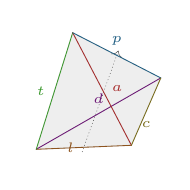
\begin{tikzpicture}[line join = round, line cap = round]

\coordinate (A) at (0.8737734,0.4020789,0.2735919); % incident to DPC (event node)
\coordinate (B) at (-0.5404401,0.6813372,-0.493664); % incident to TPA (step clocks!)
\coordinate (C) at (0.1666667,-0.787218,-0.5937256); % incident to LAC (origin anchor)
\coordinate (D) at (-0.5,-0.2961981,0.8137977); % incident to TLD (destination anchor)


% median lines: pick one
% \draw[->,color={rgb:red,1;green,1;blue,1}, densely dotted, line width = {0.2pt}] (A) -- (3*-0.2912578, 3*-0.1340263, 3*-0.0911973); % $TAL$ median
% \draw[->,color={rgb:red,1;green,1;blue,1}, densely dotted, line width = {0.2pt}] (B) -- (3*0.1801467, 3*-0.2271124, 3*0.1645547); % CDL median
% \draw[->,color={rgb:red,1;green,1;blue,1}, densely dotted, line width = {0.2pt}] (C) -- (3*-0.0555556, 3*0.262406, 3*0.1979085); % TPD median;
%\draw[->,color={rgb:red,1;green,1;blue,1}, densely dotted, line width = {0.2pt}] (D) -- (3*0.1666667, 3*0.0987327, 3*-0.2712659); % APC median;

% bimedian lines: pick one
 \draw[->,color={rgb:red,1;green,1;blue,1}, densely dotted, line width = {0.2pt}] (1.1*-0.16666665,1.1*-0.54170805,1.1*0.11003605) -- (1.1*0.16666665,1.1*0.54170805,1.1*-0.11003605); % $LP$ bimedian
% \draw[->,color={rgb:red,1;green,1;blue,1}, densely dotted, line width = {0.2pt}] (1.1*-0.1868867,1.1*-0.0529404,1.1*-0.5436948) -- (1.1*0.1868867,1.1*0.0529404,1.1*0.5436948); % $AD$ bimedian
% \draw[->,color={rgb:red,1;green,1;blue,1}, densely dotted, line width = {0.2pt}] (1.1*-0.52022005,1.1*0.19256955,1.1*0.16006685) -- (1.1*0.52022005,1.1*-0.19256955,1.1*-0.16006685); % $TC$ bimedian

% light shaded faces
\draw[-, fill={rgb:red,1;green,1;blue,1}, opacity=.05] (A)--(D)--(B)--cycle; % TDP
\draw[-, fill={rgb:red,1;green,1;blue,1}, opacity=.05] (A)--(D)--(C)--cycle; % CDL
\draw[-, fill={rgb:red,1;green,1;blue,1}, opacity=.05] (B)--(D)--(C)--cycle; % TAL
\draw[-, fill={rgb:red,1;green,1;blue,1}, opacity=.05] (A)--(B)--(C)--cycle; % APC

% color edges
\draw[-, color ={rgb:red,136;green,31;blue,147}, line width = {0.3pt}] (A)--(D); % D
\draw[-, color ={rgb:red,197;green,117;blue,43}, line width = {0.3pt}] (D)--(C); % L
\draw[-, color ={rgb:red,78;green,201;blue,59}, line width = {0.3pt}] (D)--(B); % T
\draw[-, color ={rgb:red,210;green,55;blue,55}, line width = {0.3pt}] (B)--(C); % A
\draw[-, color ={rgb:red,49;green,145;blue,201}, line width = {0.3pt}] (A)--(B); % P
\draw[-, color ={rgb:red,210;green,188;blue,45}, line width = {0.3pt}] (A)--(C); % C

% edge labels
\node[above, color={rgb:red,49;green,145;blue,201}] at (0.16666665,0.54170805,-0.11003605) {\tiny $p$}; % AB mean
\node[below, color={rgb:red,210;green,188;blue,45}] at (0.52022005,-0.19256955,-0.16006685) {\tiny$c$};  % AC mean
\node[above, color={rgb:red,136;green,31;blue,147}] at (0.1868867,0.0529404,0.5436948) {\tiny$d$};  % AD mean
\node[left, color={rgb:red,78;green,201;blue,59}] at (-0.52022005,0.19256955,0.16006685) {\tiny$t$};   % BD mean
\node[left, color={rgb:red,197;green,117;blue,43}] at (-0.16666665,-0.54170805,0.11003605) {\tiny$l$};  % CD mean
\node[right, color={rgb:red,210;green,55;blue,55}] at (-0.1868867,-0.0529404,-0.5436948) {\tiny$a$};  % BC mean

% node helper labels
%\node at (A) {\small A};
% \node at (B) {\small B};
% \node at (C) {\small C};
% \node at (D) {\small D};

\end{tikzpicture}


%     }
%    \caption{The three view axes of the independent planes map to the bimedians of the tetrahedron. The LP view axis is depicted with a gray arrow passing through the midpoints of edges $l$ and $p$. The LP plane is orthogonal to this line, here shown in translucent red plane passing through the origin. AD or TC are the other two independent planes (not shown).}
%    \label{fig:indepviewaxes}       
%\end{subfigure}
%\caption{The seven view axes of the demographic time identity map to geometric properties of the regular tetrahedron, here drawn as a perspective plot. Triad planes are seen by gazing orthogonal to a face of the tetrahedron. The independent dyad planes are seen by rotating the tetrahedron so that a pair of opposite edges are aligned at their midpoints. }
%\label{fig:viewaxes}
%\end{figure}
%
%
%
%\FloatBarrier
%\subsection*{Surface equivalencies}
%Data structured by the demographic time identity can be visualized as a surface on a Cartesian grid, where any two time measures define the abscissa and ordinate. Thus there are $\binom{6}{2}$ possible axis combinations for surfaces of this kind. Any such surface must be held constant for a third time measure. For instance, if we visualize data on a TAL plane, this is done holding a value of C, D, or P constant, for example the TAL plane of the 1915 birth cohort. For a plane defined with a triad identity, one may control for any of the remaining three measures. Independent planes can be held constant for any of the four remaining time measures: for example, the AD plane may be held constant for one of C, P, T, or L. For instance, one may view the AD plane of the 1915 birth cohort. In this case, one will notice that the TAL and AD planes for the 1915 birth cohort are different representations of the exact same set of data points.
%
%selected such that its Cartesian representation is a cross-section orthogonal to any of the seven view axes illustrated in Fig.~\ref{fig:viewaxes}. There is no reason not to do this for outcome measures, for example disease prevalence, in search of meaningful patterns. Further, when \emph{slicing} through such a complex timespace, we are agnostic about cut angles in general, but \emph{snapping} to axes defined on the basis of unit time measures leads to easier interpretation.
%
%Use this section to give a formal introduction to how a single control variable and depth implies a single surface, but the abscissa and ordinate choices can vary, implying different rotations and potentially giving different insights.
%
%This is a temporary note. I've noticed some equivalencies when taking cross-sections of the hexad timespace using the HRS data. We have four triad identities and three independent dyads. For each of these, when taking a cross-section of the 3d space, one needs to specify a control variable. For example, for APC, one could control for T, L or D. Certain combinations of abscissa, ordinate and control measure yield identical images (albeit with different axis labels due to different time measures). For example, APC, LCD, AD, and LP are all identical when controlled for T. TPD, LCD, LP, and TC are all identical when controlled for A. And in general for each of the six possible controls, there are four ways to specify a plane that will yield identically filled surfaces. By extension, we conclude that there are six *fundamental* cross sections. I deposit this text here temporarily, but this is in need of further verification, as my data filtering may need some refinement for the case of independent dyads. Specifically, for a given independent dyad we may not wish to hold one of the other four measures constant. And of course this could all be my mistake.
%

\section*{Other time points, positive and negative intervals}
Here we go beyond 
the three time points $C, P, D$ 
and beyond the assumption that $C<P<D$.

First, we can relax the assumption that $C<P<D$.
For example, Abraham Lincoln lived from 1809 to 1865.
The hundredth anniversary of his year of birth $C=1809$ was 1909.
If we take $P=1909$ and retain the earlier definition that $|T|=D-P$,
then in this case  $|T|= 1865-1909 = -44 < 0$. 
This example points out the possibility that $T<0$ if we relax the assumption that $C<P<D$.
A negative interval $T$ is to be interpreted as ``time since death'' rather that ``time until death,''
while an age $A=P-C>L$ greater than the length of life is interpreted as an anniversary of birth.
In the directed graph representation of this situation $C<D<P$, the arrow labeled $|T|$
goes from right to left, 
unlike the arrows from left to right in Fig. \ref{fig:digraph}.
The linear algebraic representation \eqref{eq:WequalsMV} of this situation requires no change
if the correct calendar dates are inserted as the values of the points.

Second, we can enlarge the set of demographic time points.
We suggest that demographic time  points fall into two categories.
The first category includes points that characterize a life regardless of the observer, 
such as $C, D$ minimally, and optionally 
the time of first marriage or entry into more or less equivalent union (denoted $M_1$), if any, 
times $M_2,\ldots$ of second and later marriages (or equivalent), if any, 
time of first ($V_1$), second ($V_2$), and later dissolutions of marriage or equivalent (V for divorce), if any, 
times $B_1, B_2, \ldots$ of first, second, and later births, if any, 
and times associated with beginnings, endings, and events of 
education $E_i, i=1,\ldots$, employment $J_i, i=1,\ldots$ (J for job), migration $G_i, i=1,\ldots$ (G for go), illness $H_i, i=1,\ldots$ (H for health) and other processes.
Some of these points, if they occur in a life,
have an order by definition, e.g., $C<D, M_i<V_i<M_{i+1}, G_i<G_{i+1}$,
while others are not ordered by definition.  
We refer generically to these $ n_1 \geq 2$ points that characterize a life
as $\pi_i, \pi_1=C<\pi_2 < \ldots < \pi_{n_1}=D$.

A second category includes points that characterize the observer or system of observation 
regardless of the life.
Examples include
the time of observation $O$,
the period $P$, and the 
times of truncation ($K_+$ when life lines begin to be reported, for example, because vital registration 
begins
and $K_{-}$  when life lines cease to be reported, for example, because vital registration ends
or because records are destroyed, 
always subject to $K_+<K_{-}$),
and perhaps others. 
We refer generically to these $n_2 \geq 0$ points that characterize the observer
as $P_i, i=1, \ldots, n_2$.



In general, for any set of $n=n_1+n_2$ points, there are ${n \choose 2}=n(n-1)/2$ pairs of distinct points.
We suppose the observer picks one point of each pair $\Delta$
as its starting point $\Delta_1$ and the other as its ending point $\Delta_2$,
thus assigning a direction to each arrow in the representation of that life by a directed graph and
a sign to its weight (length) $|\Delta|=\Delta_2-\Delta_1$.
The resulting ${n \choose 2}$ intervals are not independent 
because they are constrained by the same set of $n$ points.


\section*{Data}
Our illustrative example uses disability prevalence patterns estimated from the United States Health and Retirement Study 
(HRS) as reported in RAND version 2016v1 \citep{HRS, RAND}.
[TIM, I SUGGEST THAT WE OMIT ALL THE ``INFORMATIVE TRIADS,''
PARTLY BECAUSE YOU DISCUSSED THEM IN 2017, 
AND PARTLY TO KEEP THIS NOTE SHORT AND FOCUSED ON WHAT WE NOW CALL ``INDEPENDENT DYADS.''
IF POSSIBLE, PLEASE DEFINE THE SET OF POINTS AND INTERVALS YOU WILL EXTRACT 
FROM DATA BY USING THE NOTATION INTRODUCED IN THE PREVIOUS SECTIONS.]
To illustrate what may be learned from independent dyads,
%time perspectives can be used to take cross-sections of phenomena with multiple time dimensions. 
we estimate how the prevalence of disability varies over year of birth $C$, age $A$, and time-to-death $T$,  
only for respondents who have died, a total of 15287 individuals with a total of 82069 observations.
[TIM, DOES THIS ANALYSIS ILLUSTRATE ONE OF THE THREE HYPOTHETICAL EXAMPLES
OF INDEPENDENT DYADS DESCRIBED EARLIER? 
IF SO, PLEASE MAKE THE CONNECTION EXPLICIT HERE.
IF NOT, PLEASE EXPLAIN HOW THIS EMPIRICAL EXAMPLES RELATES TO INDEPENDENT DYADS.
THANKS!] 
Thus we have on average just over five observations per person.
The two-year spacing between survey waves implies an average trajectory length of ten years before death. 
Prevalence is defined as the average value of the disability outcome 
[TIM, CAN YOU EXPLAIN A BIT WHAT IS MEANT BY ``disability outcome''? 
IS IT A DISCRETE OR CONTINUOUS MEASURE? 
IF IT IS DISCRETE, IS IT DICHOTOMOUS OR MULTI-VALUED?
IS IT A MEASUREMENT THAT IT MAKES SENSE TO AVERAGE?]
given each combination of $C, A$, and $T$. 
Prevalence estimates are for exact midpoints in single-year intervals of $C, A$, and $T$. 
We estimate prevalence using logistic regression, where natural splines over $C, A$, and $T$ are covariates. 
The procedure takes account of the sampling structure of the HRS.
Further details can be found in \citet{riffe2017hle}. 
%Since the edges A, T, C in Fig.~\ref{fig:tet} are both connected and touch all four vertices in the graph, our smoothed prevalence fills the 3d space defined by the demographic time identity. 

%, such that we can define the remaining demographic time variables directly as follows: $P = C + A$; $D = P + T$; $L = A + T$. This lets us explore the space in a structured way using cross-section planes.

\subsection*{Availability of data and materials}
RAND HRS data are available free of charge, and require registration to download. These data are not ours to share. However, we give detailed instructions for requesting the exact source data we used here. We also include intermediate aggregate data objects to pick up part way through analyses. This repository also contains annotated \texttt{R} code to reproduce the intermediate data objects from the source data, and code for all figures and calculations from the manuscript.
The following url leads to an anonymized version of the repository, to facilitate blind review:
\url{https://url/to/anonymous/osf/repository/forthcoming}

\section*{Application}
We now explore each of the three independent dyads $\{P,L\},\{D,A\}$, and $\{C,T\}$ 
using the example of disability prevalence. 
Let $\{\tau,\Delta \}$ represent any one of the three independent dyads 
with time point $\tau$ and time interval $\Delta$. 
We use surface plots (filled contour plots) for the three distributions:
(i) raw counts $N(\tau,\Delta)$, 
(ii) counts normalized by the sum over interval lengths $N(\tau,\Delta)/N(\tau,+)$,
and (iii) counts normalized by the sum over time points $N(\tau,\Delta)/N(+,\Delta)$.
[TIM, I SUGGEST THREE FIGURES, ONE FOR EACH INDEPENDENT DYAD. 
EACH FIGURE WOULD HAVE THREE PANELS, ONE FOR EACH OF THESE THREE DISTRIBUTIONS
(i), (ii), (iii).
I AM OPEN TO YOUR SUGGESTIONS OF ALTERNATIVES.]

\section*{Discussion and conclusions}

[TO COME AFTER WE SEE THE EMPIRICAL EXAMPLE.]


%%%%%%%%%%%%%%%%%%%%%%%%%%%%%%%%%%%%%%%%%%%%%%
%%                                          %%
%% Backmatter begins here                   %%
%%                                          %%
%%%%%%%%%%%%%%%%%%%%%%%%%%%%%%%%%%%%%%%%%%%%%%

\begin{backmatter}

%\section*{Funding}
%  \censor{TR} thanks the \censor{Max-Planck-Institute for Demographic Research} for supporting this work with a fair salary. 
  
\section*{Competing interests}
  The authors declare that they have no competing interests.

\section*{Author's contributions}
  Both authors conceived of this project, undertook formal analysis, validation, drafting, and reviewing of the manuscript. TR did the data analysis, coding, visualization, and reproducibility repository curation.

\section*{Acknowledgements}
  We wish to thank N reviewers in advance for sharing their time and expertise in reviewing this manuscript. We are also thankful for comments and advice from Vanessa di Lego, Maarten Bijlsma, Jonas Sch\"oley, Alyson van Raalte, and Francisco Villavicencio.
%%%%%%%%%%%%%%%%%%%%%%%%%%%%%%%%%%%%%%%%%%%%%%%%%%%%%%%%%%%%%
%%                  The Bibliography                       %%
%%                                                         %%
%%  Bmc_mathpys.bst  will be used to                       %%
%%  create a .BBL file for submission.                     %%
%%  After submission of the .TEX file,                     %%
%%  you will be prompted to submit your .BBL file.         %%
%%                                                         %%
%%                                                         %%
%%  Note that the displayed Bibliography will not          %%
%%  necessarily be rendered by Latex exactly as specified  %%
%%  in the online Instructions for Authors.                %%
%%                                                         %%
%%%%%%%%%%%%%%%%%%%%%%%%%%%%%%%%%%%%%%%%%%%%%%%%%%%%%%%%%%%%%

% if your bibliography is in bibtex format, use those commands:
\bibliographystyle{spbasic} % Style BST file (bmc-mathphys, vancouver, spbasic).
\bibliography{references.bib}      % Bibliography file (usually '*.bib' )
% for author-year bibliography (bmc-mathphys or spbasic)
% a) write to bib file (bmc-mathphys only)
% @settings{label, options="nameyear"}
% b) uncomment next line
%\nocite{label}

% or include bibliography directly:
% \begin{thebibliography}
% \bibitem{b1}
% \end{thebibliography}

%%%%%%%%%%%%%%%%%%%%%%%%%%%%%%%%%%%
%%                               %%
%% Figures                       %%
%%                               %%
%% NB: this is for captions and  %%
%% Titles. All graphics must be  %%
%% submitted separately and NOT  %%
%% included in the Tex document  %%
%%                               %%
%%%%%%%%%%%%%%%%%%%%%%%%%%%%%%%%%%%

%%
%% Do not use \listoffigures as most will included as separate files

%\section*{Figures}
%  \begin{figure}[h!]
%  \caption{\csentence{Sample figure title.}
%      A short description of the figure content
%      should go here.}
%      \end{figure}

%\begin{figure}[h!]
%  \caption{\csentence{Sample figure title.}
%      Figure legend text.}
%      \end{figure}

%%%%%%%%%%%%%%%%%%%%%%%%%%%%%%%%%%%
%%                               %%
%% Tables                        %%
%%                               %%
%%%%%%%%%%%%%%%%%%%%%%%%%%%%%%%%%%%

%% Use of \listoftables is discouraged.
%%
%\section*{Tables}
%\begin{table}[h!]
%\caption{Sample table title. This is where the description of the table should go.}
%      \begin{tabular}{cccc}
%        \hline
%           & B1  &B2   & B3\\ \hline
%        A1 & 0.1 & 0.2 & 0.3\\
%        A2 & ... & ..  & .\\
%        A3 & ..  & .   & .\\ \hline
%      \end{tabular}
%\end{table}

%%%%%%%%%%%%%%%%%%%%%%%%%%%%%%%%%%%
%%                               %%
%% Additional Files              %%
%%                               %%
%%%%%%%%%%%%%%%%%%%%%%%%%%%%%%%%%%%

%\section*{Additional Files}
%  \subsection*{Additional file 1 --- Sample additional file title}
%    Additional file descriptions text (including details of how to
%    view the file, if it is in a non-standard format or the file extension).  This might
%    refer to a multi-page table or a figure.

%  \subsection*{Additional file 2 --- Sample additional file title}
%    Additional file descriptions text.


\end{backmatter}
\end{document}


% TR: deprecate enture Quebec section, because we only produced
% flattened surfaces, which although they contain patterns that are
%fun to interpret, half of them are due to boundary conditions
% that introduce tricky kinds of heterogeneity. We therefore
% would like to focus on controlled cross-sections of the 3d demographic
% timespace.


%\section*{Independent time surfaces of population structure}
%As a first pass to demonstrate concepts, we cross-tabulate Qu\'{e}bec's historical population structure by the three sets of independent demographic time measures. Each cross-tabulation is represented as a demographic surface using filled contour heat maps to create Lexis-like surfaces. These surfaces are distinct from Lexis surfaces in a few important ways. Lexis surfaces are drawn with diagonal lines at a slope equal to the aspect ratio between time units in $y$ and time units in $x$, usually 45$^\circ$ (APC, LCD). Other triad time surfaces might be drawn with descending diagonals (TPD, TAL). Surfaces on independent planes might have features that run horizontally, vertically or in both 45$^\circ$ and -45$^\circ$ diagonals, depending on the case, but in general it only makes sense to draw them as a standard Cartesian grid without any diagonals, although they could be drawn with diagonals running in both directions. 

%As mentioned, the three independent dyads in the demographic time identity each consist in one event measure and one duration measure. Our convention for orienting the Cartesian plane is to use the date measure as abscissa ($x$-axis) and the duration measure as ordinate ($y$-axis). Since a duration measure is the difference between two event dates, this means that independent dyads in this particular identity only arise when three event dates are known, which identifies the full demographic time identity (PCD implies TAL). Tabulations by two independent time measures can only be done in practice if each of the six demographic time measures are either observed or derivable. 

%\subsection*{LP: Lifespan and period}
%Following this standard orientation, we draw an LP diagram with period in abscissa and lifespan in the ordinate axis. This is an ageless diagram. An individual with a lifespan of 80 years is represented as a horizontal line spanning from the time of birth until the time of death. That is, for each increment in P, L is uniform within an individual. An individual lifespan, which determines the ordinate, is only known in retrospect. On a single lifeline, one can trace the progression of age (and the other time measures) from left to right.  Fig.~\ref{fig:lpd} shows an example of an LP diagram that includes some illustrative lifelines. The lifeline labelled \textbf{A} is in a lower ordinate position because it represents a shorter life, whereas the lifeline \textbf{B} represents a longer life. These example lifelines do not overlap, but for aggregate data tabulated by L and P, any given coordinate contains a mixture of ages. Heterogeneity of this kind is greater for longer lives than for shorter lives.

%REDO figure for HRS, note to self.
%\begin{figure}
%\centering
%\includegraphics[scale=.7]{Figures/LPdiagram.pdf}
%\caption{LP diagram, with example lifelines. Lifeline \textbf{A} starts with a birth (solid circle) in 1836, and ends with a death (crossed circle) in 1849. Lifeline \textbf{B} starts with a birth in 1940, and ends with a death in 2023. The ordinate position L is equal to the length of each life.}
%\label{fig:lpd}
%\end{figure}

%Fig.~\ref{fig:lpq} displays the Qu\'{e}bec population structure on an LP surface. Higher $y$ values correspond to longer lives, and therefore more overlapped underlying lifelines. The upper regions of the surface are thus smoother with respect to time than lower regions. Growth over time in to-be-long-lived individuals could occur due to population growth or mortality improvement. We know this pattern is not due to migration because this population was mostly closed in this time. For Qu\'{e}bec, increasing contours over time are primarily due to population growth. 

%Shorter lives (lower L) reveal the rhythms of mortality, adding a peculiar relief to the surface. High-mortality years are marked with vertical cliffs in population structure: Right-aligned cliffs are found on the LP surface when many lives over a range of ages are simultaneously extinguished. These vertical rifts trace back to births over a range of years, producing the -45$\circ$ feature \includegraphics{Figures/LP_mort_tri.pdf}. Mortality shocks therefore produce raised triangle relief pattern in population structure. A single isolated year with an extremely high number of births could produce a raised left-edge, but fertility shocks of this kind are far less prominent than mortality shocks in this population. Some known epidemics are marked below the surface with red strips \citep[cf Figure 1.1][]{mazan2011} 

%\begin{figure}
%\centering
%\includegraphics[scale=.9]{Figures/QuebecLP.pdf}
%\caption{Population structure by length of life and year. %Logged counts}
%\label{fig:lpq}
%\end{figure}

%The inverted step pattern on the right edge of this surface betrays some of the peculiarities of data collection for this source. Death information comes from burial records, which had some age constraints in data collection, depending on the period: For years 1800 to 1825 only deaths in ages 50 and greater were collected. For years 1826 to 1850, only deaths in ages 75 and greater were collected. Exceptions to this block edge structure owe to the use of multiple potential sources for death dates. Since lifelines accrue to the LP surface only after deaths occur, the right-side region of Fig.~\ref{fig:lpq} is incomplete: further increments will happen as death data are added to the series. This incompleteness is less for shorter lives, which accrue quickly to the surface due to their brevity.

%\FloatBarrier
%\subsection*{TC: Time-to-death and cohort}

%The time-to-death T distribution of an extinct and closed birth cohort C (defined as a birth cohort all members of which have died) reveals its life table. Fig.~\ref{fig:tcd} shows an example of a TC diagram, where C is in abscissa and T is the ordinate variable. A lifeline on the CT plane is drawn as a vertical segment extending downward from birth until death on the bottom axis. For example, lifeline \textbf{A} represents an individual born in 1624 and dying at age 20 in 1644. In an aggregate of population exposure, this lifeline contributes 1 to the count in each time step descending from 20 to 0 --- the entire countdown timeline. Since each member of a birth cohort eventually comes to die, the coordinate $T = 0$ is maximally heterogeneous with respect to any of the other demographic time measures (A,L,P,D), and lifeline overlap decreases in higher T.

%\begin{figure}
%\centering
%\includegraphics[scale=.6]{Figures/TCdiagram.pdf}
%\caption{TC diagram, with example lifelines. Lifeline \textbf{A} is from the 1624 birth cohort, and starts with a birth (solid circle) with 20 remaining years of life, and ends with a death (crossed circle) on the bottom axis (year 1644). Lifeline \textbf{B} is from the 1638 birth cohort, starting with 94 remaining years of life at birth, and ending with death in 1732.}
%\label{fig:tcd}
%\end{figure}

%Fig.~\ref{fig:tcq} shows a TC tabulation of the Quebec population structure. A few features of this surface stand out. First, as a cohort ages, vertical strips are completed upwards. Ergo, the lower regions of the surface are more complete than the upper regions, and the slanted step structure on the right edge of the surface corresponds to the block-step pattern of the LP surface in Fig~\ref{fig:lpq}. Second, the relatively sparse earlier cohorts are visible as vertical strips. This pattern is due to left-censoring on the moment of migration. As the series progresses rightward the cohort experience becomes more completely described in the closed population renewal, making the series smoother. In general, we see the population grow as birth year advances. If one were to normalize cohort size to something constant then the surface would closely resemble an AC Lexis surface of survivorship.

%\begin{figure}
%\includegraphics[scale=.9]{Figures/QuebecTC.pdf}
%\caption{Population structure by time to death and birth cohort.}
%\label{fig:tcq}
%\end{figure}

%\FloatBarrier
%\subsection*{AD: Age and year of death}

%Following our convention, we draw an AD diagram with year of death D in the abscissa and age A in the ordinate. Lifelines in the AD diagram start at age 0 on the bottom axis, and rise vertically until the age at death, always within the same death cohort D. The AD diagram is therefore the reverse of the TC diagram: Fig.~\ref{fig:add} uses the same lifelines as Fig.~\ref{fig:tcd}. Thus the lifeline \textbf{A} starts at age 0 and rises until death at age 20 in 1644 (D). D is constant for an individual in this diagram. In the TC diagram the line for the same life was drawn 20 years earlier in the year of birth, and the lifeline descends rather than rises. 
%\begin{figure}
%\centering
%\includegraphics[scale=.6]{Figures/ADdiagram.pdf}
%\caption{AD diagram, with example lifelines (same as in previous diagrams). Lifeline \textbf{A} is destined to die in 1644, starting with a birth (solid circle) at age 0, and ending with a death (crossed circle) on at age 20. Lifeline \textbf{B} is destined to die in 1732, starting at age 0 and rising to a death at age 94 in 1732.}
%\label{fig:add}
%\end{figure}

%In a population aggregate, exposure accrues as in the other diagram settings: lifelines contribute 1 year to exposure in each year over the lifecourse. There is no direct way to infer a life table from an AD population structure unless the population happens to be in stationary renewal \citep{villavicencio2016symmetries}, and in this narrow case the TC surface would appear identical to the AD surface. Fig.~\ref{fig:adq} shows an AD tabulation of the same Qu\'{e}bec data. Whereas vertical striation in the TC tabulation of Fig.~\ref{fig:tcq} was primarily due to birth cohort size, in Fig.~\ref{fig:adq} vertical striation results from mortality shocks. Dark vertical lines in this surface correspond to the right edge of the \emph{mortality triangles} of the LP surface. Light vertical strips might be due to stochasticity and sparseness in early years, to under-coverage or under-registration of deaths in particular years, or to selection following large mortality shocks \citep{luy2019life}. The surface has a hard right edge because the source data collection ceases around 1850, but recall from the LP surface that different age ranges were collected until different final years. Since deaths for the years 1826 to 1850 were only collected for ages 75+, the AD surface is flat in ages 0 to 74 for these same years. Likewise the preceding quarter century will be flat for age 0 to 49. [[[Tim, what accounts for the vertical darker strips in these time intervals?]]] The AD surface of Fig.~\ref{fig:adq} is therefore incomplete in the area corresponding to the white space below the stepped right edge of Fig.~\ref{fig:lpq}.

%\begin{figure}
%\includegraphics[scale=.9]{Figures/QuebecAD.pdf}
%\caption{Population structure by age and year of death.}
%\label{fig:adq}
%\end{figure}

%\FloatBarrier
%\section*{Independent time surfaces as cross-sections}
%Here use example of HRS prevalence surfaces produced at novel \emph{cut} angles. I'm thinking maybe small multiples, since each would be a fly-through of cross sections in fixed intervals. There would be 3 independent fly-throughs, and 4 Lexis-like fly throughs. These would be  like Fig.~(7) of \cite{riffe2017demographictime}, which is a fly-though at the TAL viewing angle. So, maybe each fly-through is a column and each perspective is a row? Maybe 10-year jumps in columns to imply 3-4 columns? Total? For example, each TAL slice in that Fig 7 is held for a fixed C. It would have been possible to hold P or D fixed instead, but I guess the actually slices would be identical, just the labels would change. Just need to be clear about it when labelling said panel figure.
